\documentclass[a4paper,12pt]{extarticle}
\usepackage[margin=2cm]{geometry}
\usepackage[parfill]{parskip}
\usepackage[utf8]{inputenc}
\usepackage{hyperref}
\usepackage{multicol}
\usepackage{graphicx}
\usepackage{fancyhdr}
\usepackage{xcolor}

\def\LayoutTextField#1#2{#2}
\def\LayoutCheckField#1#2{#2}

\begin{document}


\pagestyle{fancy}
\fancyhead{}
\fancyhead[LO,LE]{\textbf{Locations}}
\fancyhead[RO,RE]{\textbf{Scouts de l'Abbaye de Bevaix}}
\fancyfoot{}
\fancyfoot[RO,RE]{\thepage}
\fancyfoot[LO,LE]{Révision du 05/01/2024}


\begin{titlepage}
    \begin{center}
        \Huge Contrat de location du chalet

        \vspace{3cm}
        \includegraphics{../../logos/Logo_Abbaye_500.png}
        \vspace{3cm}

        \huge Groupe scout de l'Abbaye, Bevaix 
    \end{center}
\end{titlepage}


\section{Information locations}

Le local que nous mettons à disposition dispose d'une surface d'environ 40 $m^2$ et peut accueillir une trentaine de personnes.
La location comprend entre autres la mise à disposition de la cuisine, des sanitaires, des tables, des chaises et un fourneau à bois, ainsi que du bois pour ce dernier.

Des dortoirs peuvent également être loués, de manière supplémentaire.
Ces derniers peuvent accueillir 8 personnes sur des matelas (quelques couvertures militaires sont aussi mises à disposition).

Le montant de la location sera versé au plus tard une semaine avant la location. La taxe de séjour, exigée par le canton de Neuchâtel, s'élève à CHf 3.20 par nuit et par personne majeure séjournant dans le local.

La caution s'élève à CHF 300.00 et est payable en même temps que le prix de location. Une preuve de paiement sera jointe au contrat. La caution sera restituée après l'état des lieux dans la mesure où les locaux sont rendus conformément au règlement. Le montant de la taxe de séjour est déduite de la caution.

Nous vous rendons attentif au fait qu'aucun élément de nettoyage, tel que des sacs poubelle, des linges et autre produits de nettoyage ne sont mis à disposition (vous trouverez toutefois des seaux et des balais).

Plus d'informations et des images des lieux dans la rubirque location du site \url{https://scouts-bevaix.ch}

\newpage

\section{Règlement de location \label{sec:contract}}

\subsection{But}
Le but du présent règlement est d'assurer une utilisation du chalet conforme aux intérêts du Groupe Scout de l'Abbaye. Ceci vise à maintenir le bon état d'entretien du bâtiment et de ses alentours.

\subsection{Comité du chalet des Scouts}

Le Groupe Scout de l'Abbaye, constitué en association au sens des articles 60 et suivants du Code Civil Suisse, décide que le comité a pour tâche la gestion et l'administration du chalet. Il en établit le règlement et fixe les tarifs d'utilisation. 
La gestion des locations est confiée à une gérante qui est directement subordonnée au comité.

\subsection{Utilisateurs}
Le chalet est destiné, en premier lieu, à abriter les activités du Groupe Scout de l'Abbaye.
Il peut en outre être mis à disposition d'autres groupes scouts, notamment pour des camps et des cours de formation. En dernier usage, il peut être loué à des tiers ou sociétés qui s'engagent à respecter les lieux et le présent règlement.

\subsection{Location}

Le chalet est loué, principalement, pour des soirées ou des après-midis.
Pour toute autre demande, comme des camps ou des week-ends, veuillez contacter le Groupe par mail à l'adresse suivante : locations@scouts-bevaix.ch

{\color{red} Les locaux ne seront, en principe, pas loués pendant les séances du Groupe (samedi, de 13h30 à 17h30) ainsi que lors de camps. En cas d'arrivée lors d'une séance, avant 17h30, les locaux vous seront refusés). }

\subsection{Paiements}
Les sommes dues pour les locations seront versées sur le compte suivant :

CH11 8080 8006 8235 9023 0 \\
Compte d'association \\
Titulaire : Groupe Scout de l'Abbaye, Charcottet 10, 2022 Bevaix \\

\subsection{Annulation}

Vous êtes priés de nous faire part de votre décision d'annulation au minimum 1 semaine avant la date fixée.
Si vous n'arrivez pas à tenir ce délai, nous retiendrons, au remboursement de la location, un montant d'annulation tardive comme stipulé dans le contrat.

\subsection{Responsable}
La personne signataire du contrat doit être majeure et sera tenue responsable des clauses du contrat, qu'elle devra respecter et faire respecter.
Elle devra être présente à la remise des clés et lors de l'état des lieux. Elle sera tenue pour responsable de la conduite des utilisateurs.
La consommation d'alcool par des mineurs ainsi que l'usage de stupéfiants sont formellement interdits.

\subsection{Respect des locaux}
Les utilisateurs prendront soin des locaux et des installations.
Les armoires fermées à clef ainsi que les locaux du matériel et celui des chefs ne sont pas destinés à l'usage des locataires.
Ces derniers seront tenus de réparer les dommages qu'ils pourraient avoir causés.
De plus {\color{red} il est strictement interdit de fumer à l'intérieur des locaux.}
Si la moindre suspicion existe (odeur, mégots, …) un prélèvement de 150.- sera imputé sur la caution.

\subsection{Respect du voisinage}
La propreté des alentours et la quiétude de la forêt devront être respectées.
Il est interdit de piétiner l'herbe du pâturage aux alentours et de couper du bois vert.
A l'extérieur, le feu ne doit être fait qu'à l'emplacement prévu (du bois peut être mis à disposition sur demande).
Seuls 2 véhicules sont admis à proximité du chalet (ils seront stationnés sur la place prévue à cet effet, coté Neuchâtel), les autres véhicules seront stationnés sur le parc asphalté près du stand de tir. Cette mesure est imposée afin de permettre la manoeuvre d'une ambulance.

\subsection{Remise et rendu des clés (état des lieux)}
Les clés seront remises selon accord avec la gérante (rendez-vous à fixer).
{\color{red} L'état des lieux se fait à la fin de la location} soit à 17h lors d'une location en après-midi et à 11h le lendemain pour une location le soir.
Le chalet sera rangé et nettoyé aux heures dites. Les volets et fenêtres seront fermés et les lumières éteintes.
{\color{red} Des pénalités seront perçues en cas de retard.
En cas de perte ou de vol de la clé de location, la personne responsable s'engage à remplacer, à ses frais, la totalité du système de verrouillage des locaux loués.
Si des dégâts sont constatés, le montant sera prélevé sur la caution. Si les montants sont supérieurs à la caution, les montants en question seront demandés à la personne responsable.}


\subsection{Dispositions particulières}

\begin{itemize}
\item La consommation d'eau est comprise dans le prix de location.
L'eau chaude est limitée à la capacité du chauffe-eau.

\item Suivant la nature et la durée de la location, le compteur pourra être relevé avant et après la location.
L'électricité pourra être facturée en sus selon la consommation effective.

\item Un fourneau à bois permet le chauffage des locaux. Le bois de feu se trouve dans un bûcher à côté du fourneau.
Les utilisateurs veilleront à ne pas entreposer des objets inflammables à proximité du fourneau en fonction.

\item Un dortoir de huit places est aménagé. Les locataires doivent apporter leurs draps
ou leurs sacs de couchage. Quelques matelas en plus permettent d'aménager la salle
en dortoir.

\item Il est obligatoire qu'un extincteur soit présent dans la salle selon les normes incendie.
En cas d'utilisation abusive, la recharge sera facturée Frs 250.00.

\item La cuisine est équipée d'un frigo, d'une cuisinière électrique à quatre plaques.
La vaisselle est prévue pour une trentaine de personnes (elle est cependant un peu vétuste).
Les pattes à laver, linges à vaisselle, serpillières et produits de nettoyage seront apportés par les utilisateurs.
Pour des raisons d'hygiène les restes de nourriture devront être emportés.

\item Les locataires apporteront leur papier hygiénique et des sacs à poubelles officiels sac Neva (sac gris).
Ils veilleront à la propreté et à l'aération des toilettes.
Une douche peut être ouverte sur demande.

\item Les sacs d'ordures devront être déposés dans les containers officiels disposés en contrebas au bord de la route.

\item Tout acte de nature à troubler la tranquillité publique est interdite. Le bruit est à éviter entre 22h00 et 06h00.

\item En cas de manifestation à l'extérieur, des tables et des bancs peuvent être mis à disposition.

\item Si un des éléments cités dans le contrat n'est pas respecté, la ristourne de la caution sera réduite.
\end{itemize}

\subsection{Règlements et lois établis par la Confédération et le Canton}
La personne responsable garantit le respect des règlements et autres lois établis par la Confédération et le canton, notamment en ce qui concerne les restrictions de personnes et autres règles concernant les rassemblements de personnes.

Arthur Chapuis, président du groupe scout de l'Abbaye, 12.12.2021, rév. mars 2024 NH

\newpage

\section*{Contrat de location}

Ce document fait office de contrat de location.
Le contrat doit être retourné signé (par mail ou par courrier) et payé {\color{red}au plus tard une semaine avant la location.}
Il doit être transmis à l'adresse mail locations@scouts-bevaix.ch
Le contrat sera accompagné de la preuve de paiement. (voir site web \url{https://scouts-bevaix.ch}) 

La personne signataire du contrat doit être majeure et sera tenue responsable des clauses du contrat, qu'elle devra respecter et faire respecter. Elle devra être présente à la remise des clés et lors de l'état des lieux et sera tenue pour responsable de la conduite des utilisateurs.

Compte pour le versement: \textit{Voir page suivante}

\subsection*{Responsable location}

\noindent\begin{tabular}{@{}l l}

Prénom, Nom & \TextField[width=10cm]{prenom_nom} \\
Date de naissance & \TextField[width=10cm]{naissance} \\
Rue & \TextField[width=10cm]{rue} \\
Localité & \TextField[width=10cm]{localite} \\
N° de tél. (portable) & \TextField[width=10cm]{tel} \\

\end{tabular}

\subsection*{Location}

Location du \TextField[width=4cm]{debut} au \TextField[width=4cm]{fin}

Cocher les cases qui vous correspondent:

\begin{itemize}
    \item[] \CheckBox[]{midi} + 180 CHF : Location locaux de 11h30 à 17h30 (après-midi)
    \item[] \CheckBox[]{soir} + 180 CHF : Location locaux de 17h30 à 11h30 (soir et matin)
    \item[] \CheckBox[]{dortoirs} + 50 CHF : avec dortoirs
\end{itemize}

+ 300 CHF de caution rendue ultérieurement en fonction de l'état des lieux à la fin de la location.

La taxe de séjour s'élève à CHf 3.20 par nuit et par personne majeure séjournant dans le local.
En cas d'annulation à moins de 1 semaine de la date fixée, 30 CHF seront retenus.

La réservation sera confirmée dès réception du présent contrat, dûment signé, accompagné de la preuve de paiement.


\CheckBox[]{cbx} J'ai lu et compris le réglement de location (Section~\ref{sec:contract}).


Lieu et date: \TextField[width=10cm]{date}

Signature de la personne responsable: \hrulefill

\newpage

Compte pour le versement:

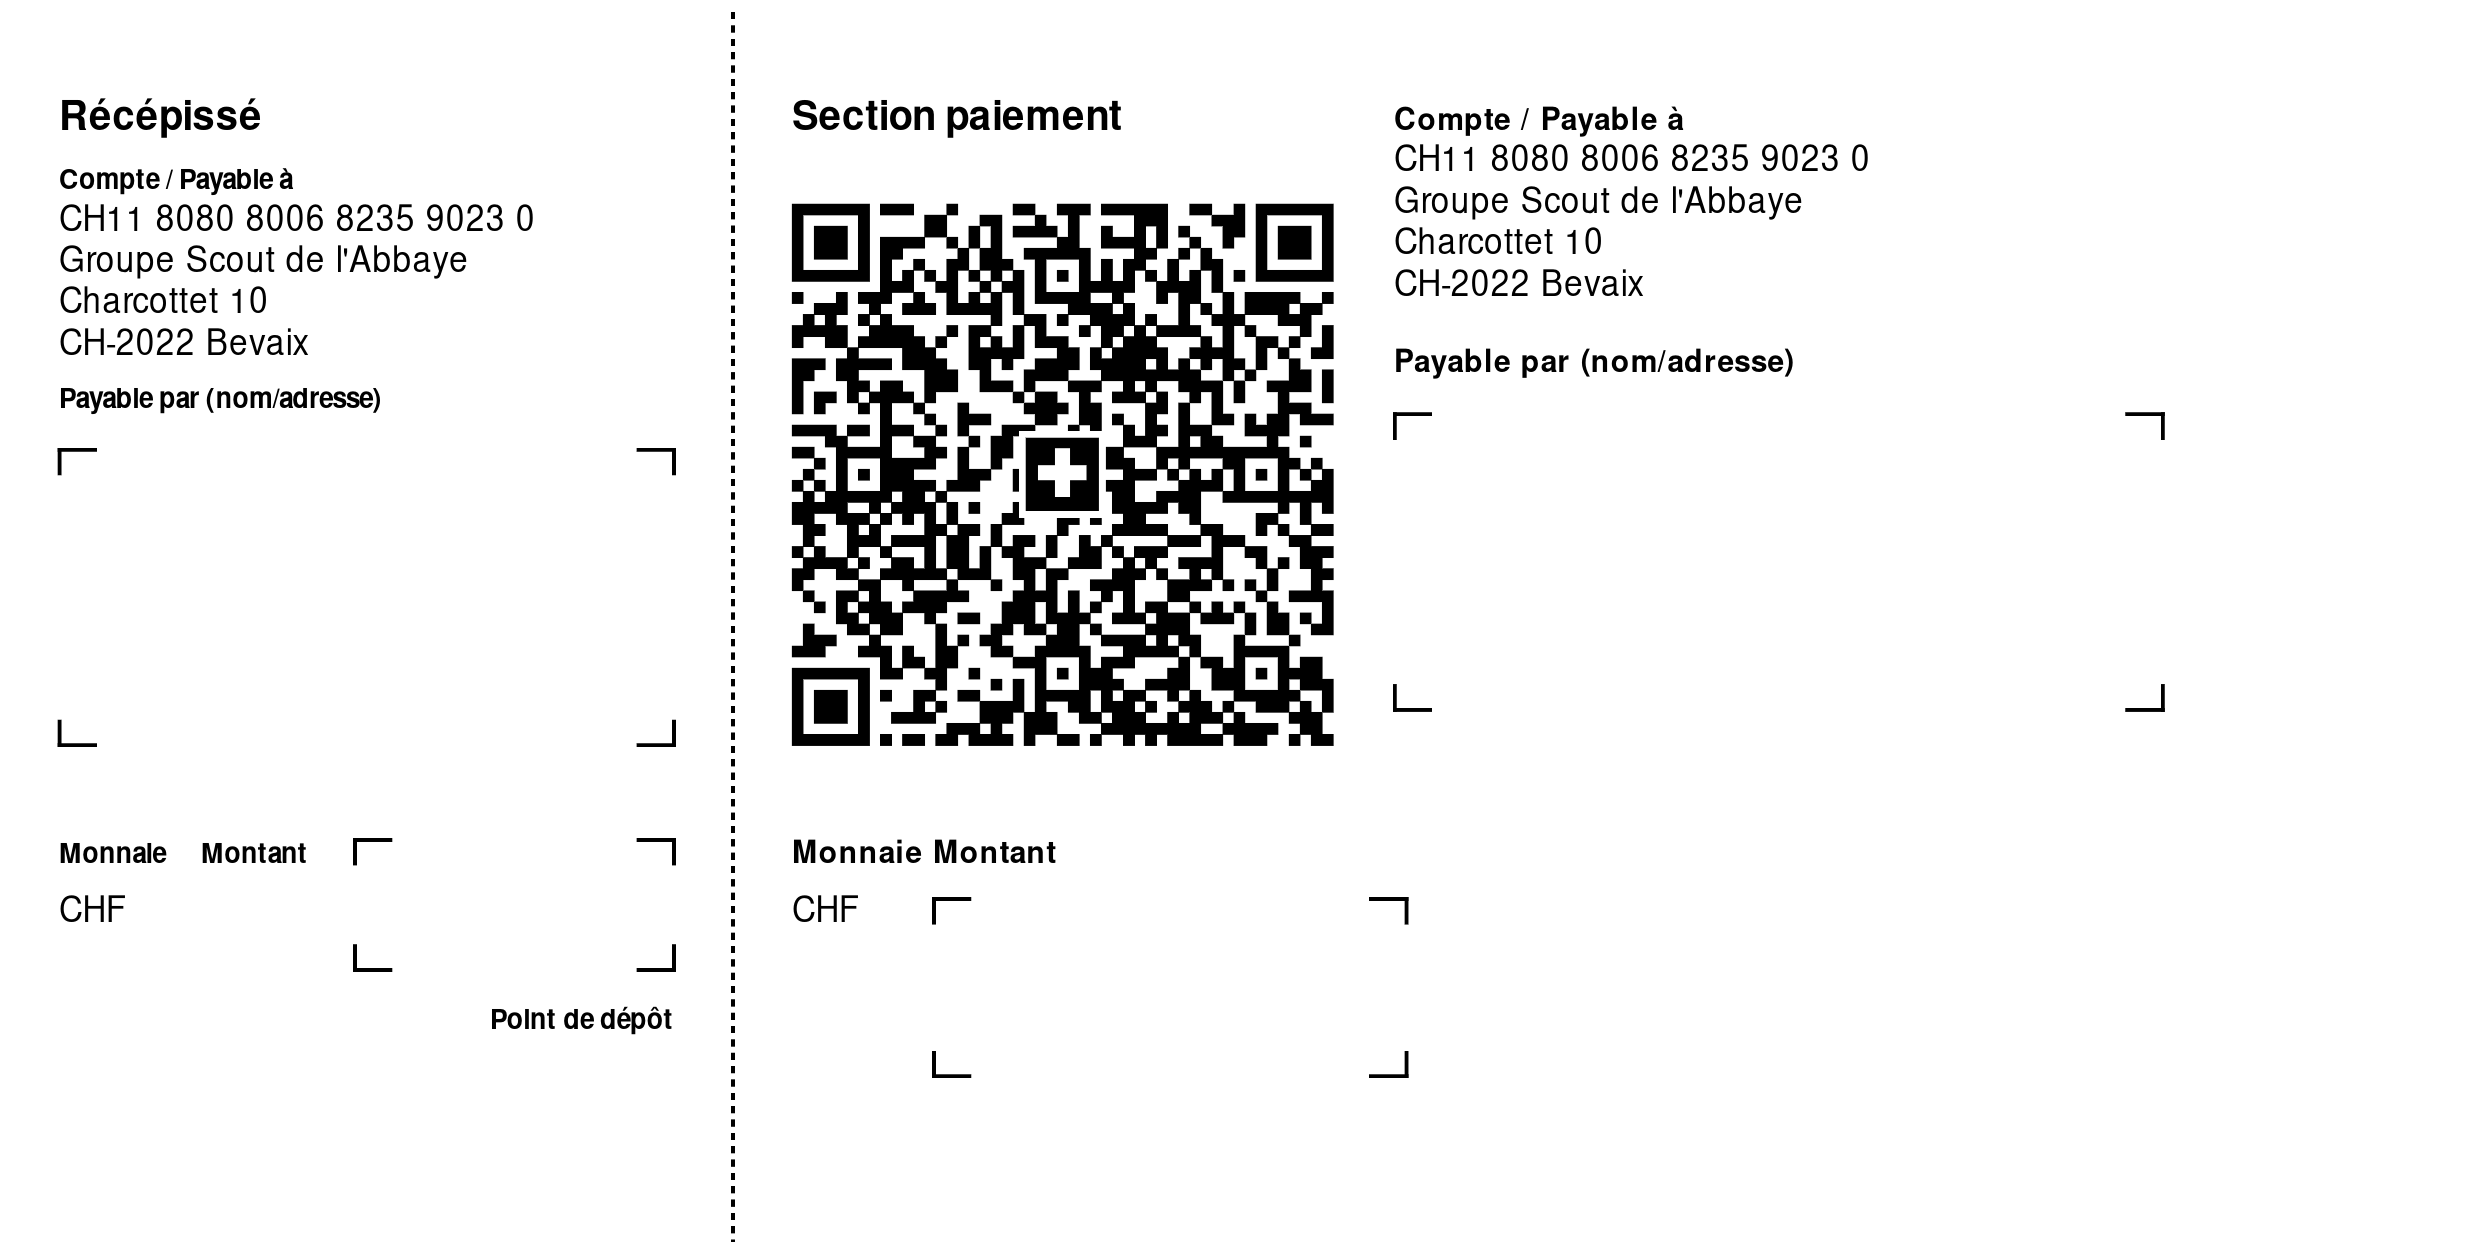
\includegraphics[width=18cm]{../../misc/qrbill.png}

\end{document}
